\documentclass{standalone}
%
\usepackage{tikz}
\usetikzlibrary{backgrounds,shapes.callouts}
\usepackage{tkz-euclide}
\usepackage{xcolor}
\usepackage{ifthen}
%
\definecolor{space}{HTML}{1F2C4E}
\definecolor{earth}{HTML}{0089FA}
\definecolor{dida}{HTML}{FFDE00}
\definecolor{title}{HTML}{FBA706}
\definecolor{moon}{HTML}{AFAFAF}
%
\usepackage{fontspec}
\setmainfont{Open Dyslexic}
%
\title{Una storia illuminante}
\begin{document}
	\tikzset{
		partial ellipse/.style args = {#1:#2:#3}{insert path={+ (#1:#3) arc (#1:#2:#3)}},
		notice/.style  = { draw, ellipse callout, callout relative pointer={#1} },
	}
	\begin{tikzpicture}[background rectangle/.style={fill=white},show background rectangle,>={[inset=0,angle'=27]Stealth}]
		%title
		\draw [black,ultra thick,fill=title] (0,9.8) rectangle (30,16.8);
		\node at (15,14.8) {\textcolor{black}{\fontsize{90}{91}\selectfont Una storia}};
		\node at (15,11.8) {\textcolor{black}{\fontsize{90}{91}\selectfont illuminante}};
		%
		\begin{scope}[shift={(0,5)}]
			\draw [ultra thick, fill=earth] (20.5,4) rectangle (25.5,-4);
			\node at (23,0) {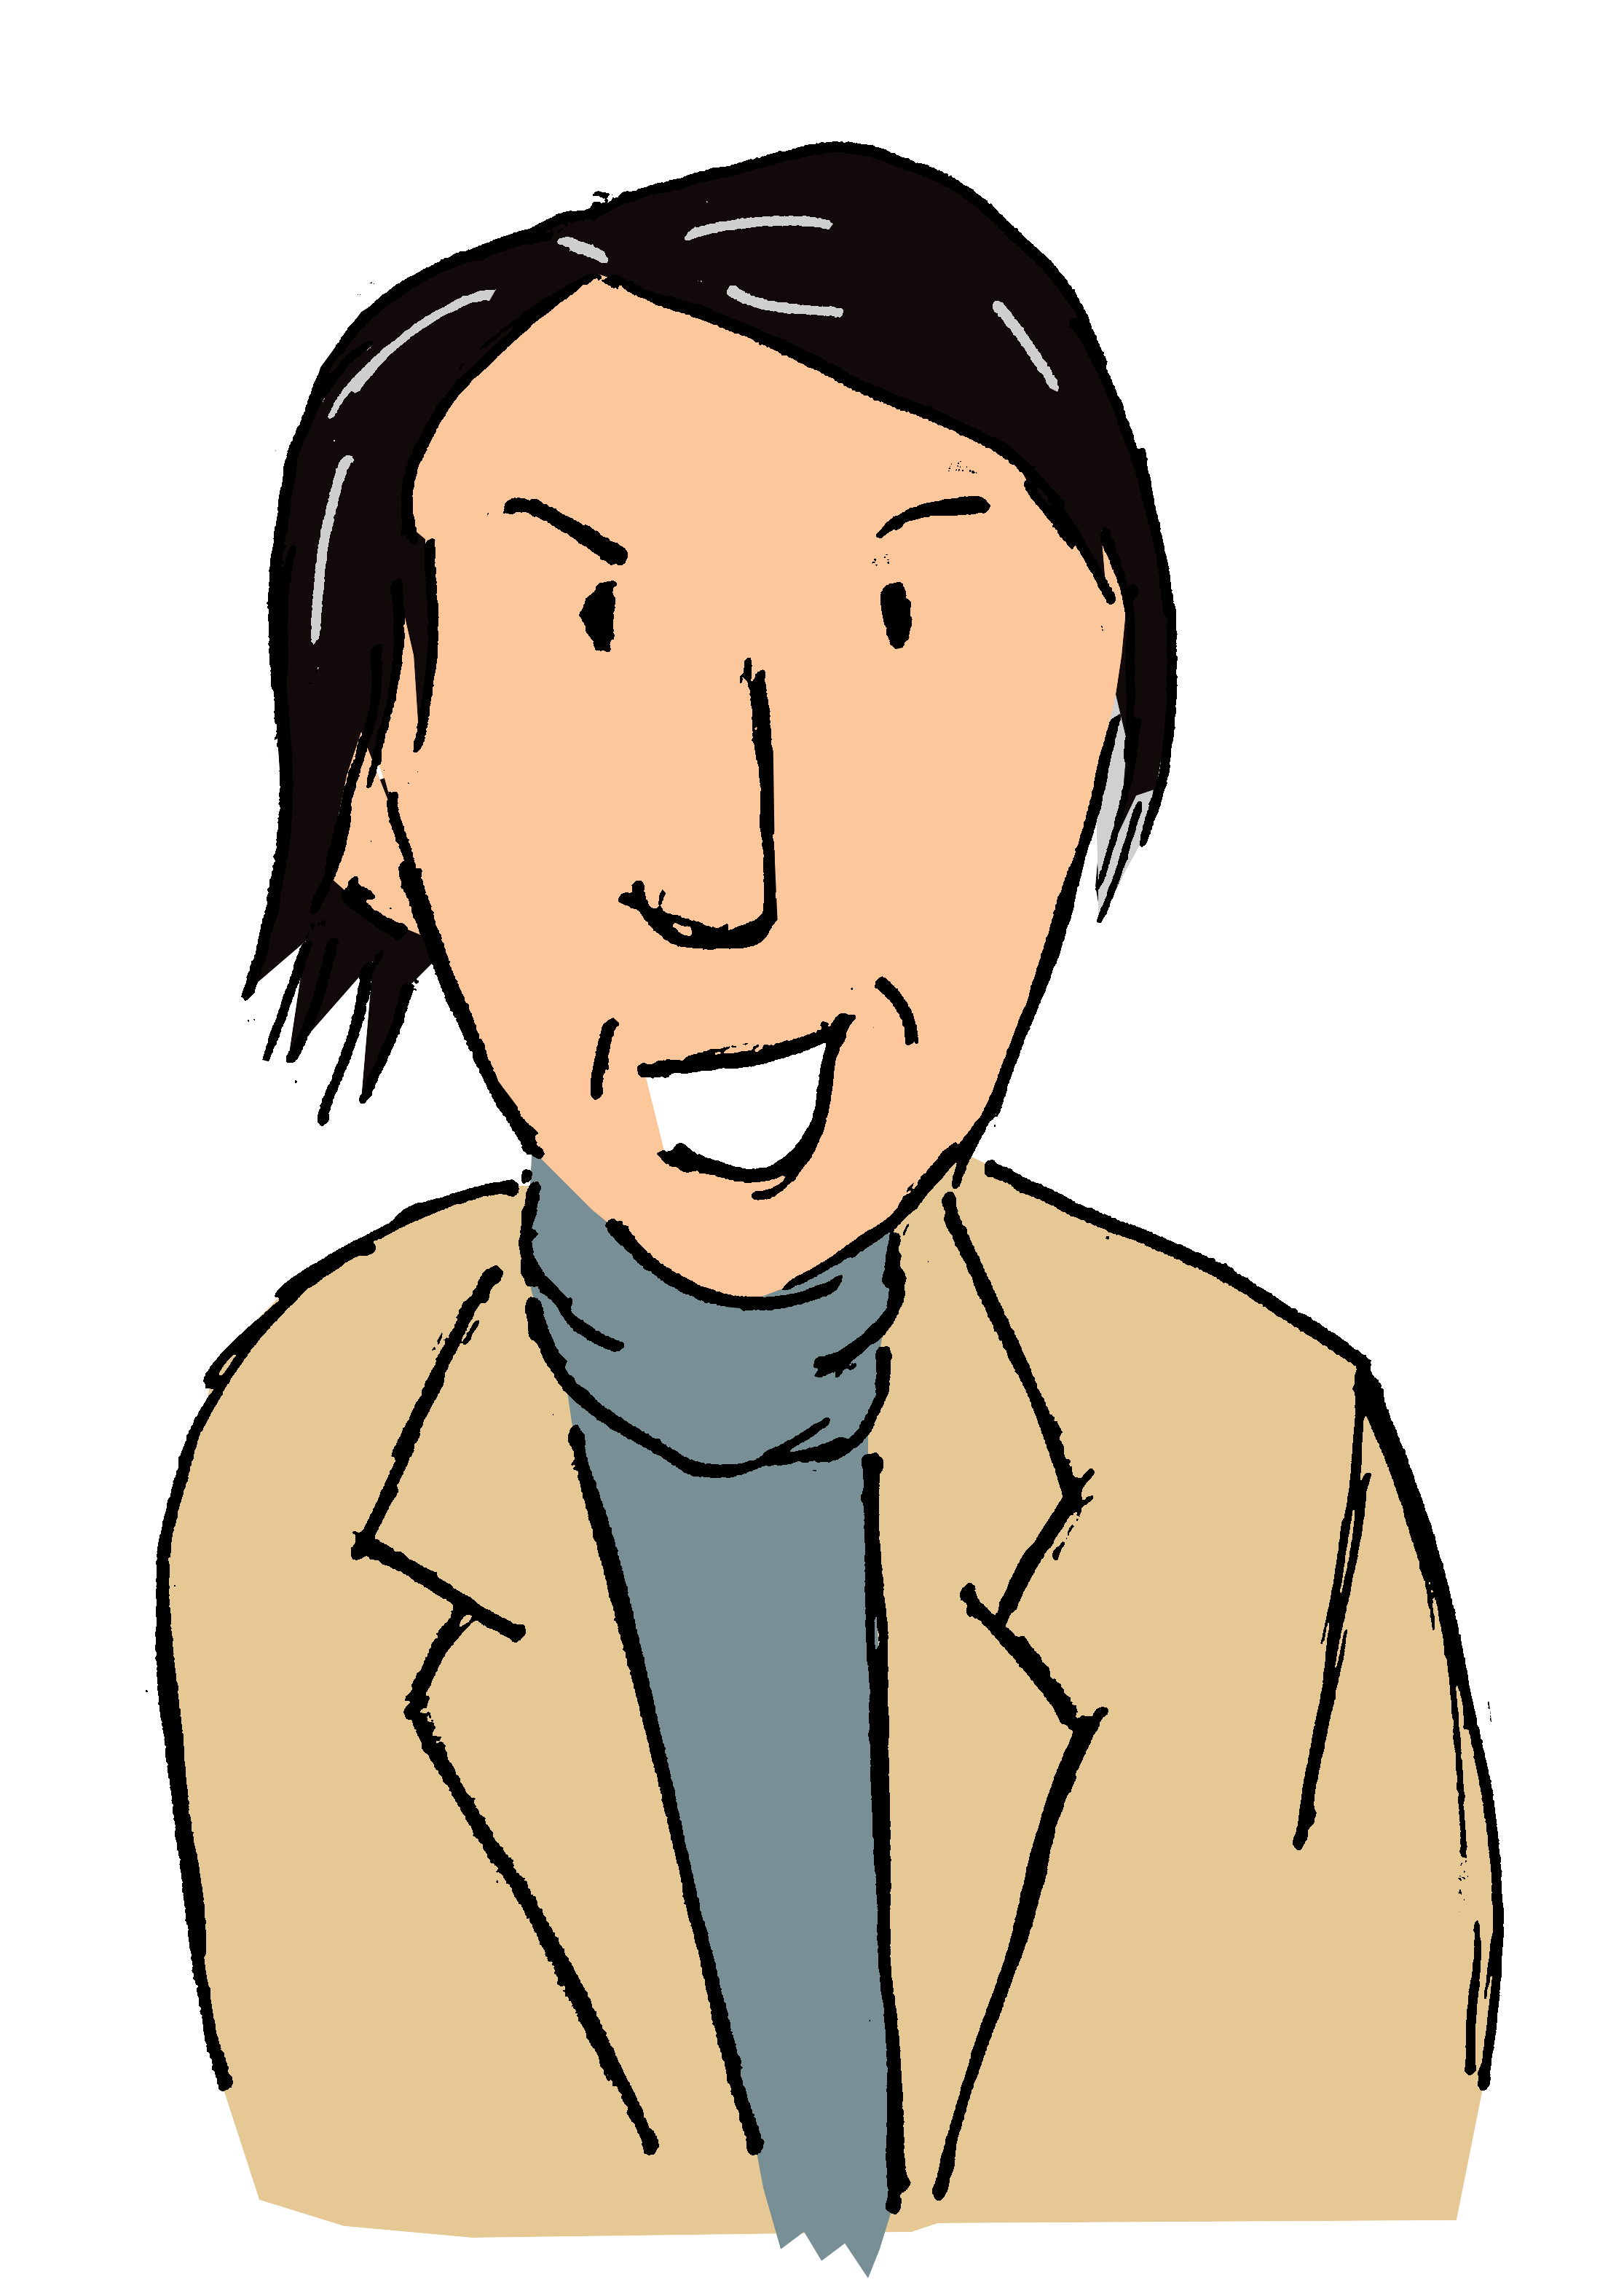
\includegraphics[width=5cm]{carl_sagan}};
			\node (example-textwidth-2) [notice={(3,0.5)}, ultra thick, right, align=center, text width=12cm, color=black, fill=white, font=\fontsize{23pt}{24pt}\selectfont] at (1,-1) {Uno degli assunti fondamentali per la teoria della relatività di \textbf{Albert Einstein} e della fisica è la costanza della velocità della luce. Vediamo la storia della misurazione del suo valore.};
		\end{scope}
		%
		\begin{scope}[shift={(0,-2)}]
			\draw [ultra thick, fill=dida] (2.5,0) rectangle (28,-4);
			\node (example-textwidth-2) [right, align=left, text width=25cm, color=black, font=\fontsize{18pt}{19pt}\selectfont] at (3,-2) {Il primo a proporre una teoria della luce che prevedesse un valore finito per la sua velocità fu il greco \textbf{Empedocle}, ma non fece mai alcun vero tentativo per misurarne il valore. Il primo a proporre un esperimento per questo scopo fu \textbf{Galileo Galilei}.};
		\end{scope}
		%
		\begin{scope}[shift={(0,-14)}]
			\fill [yellow] (5,5.7) rectangle (27,5.8);
			\node at (5,0) {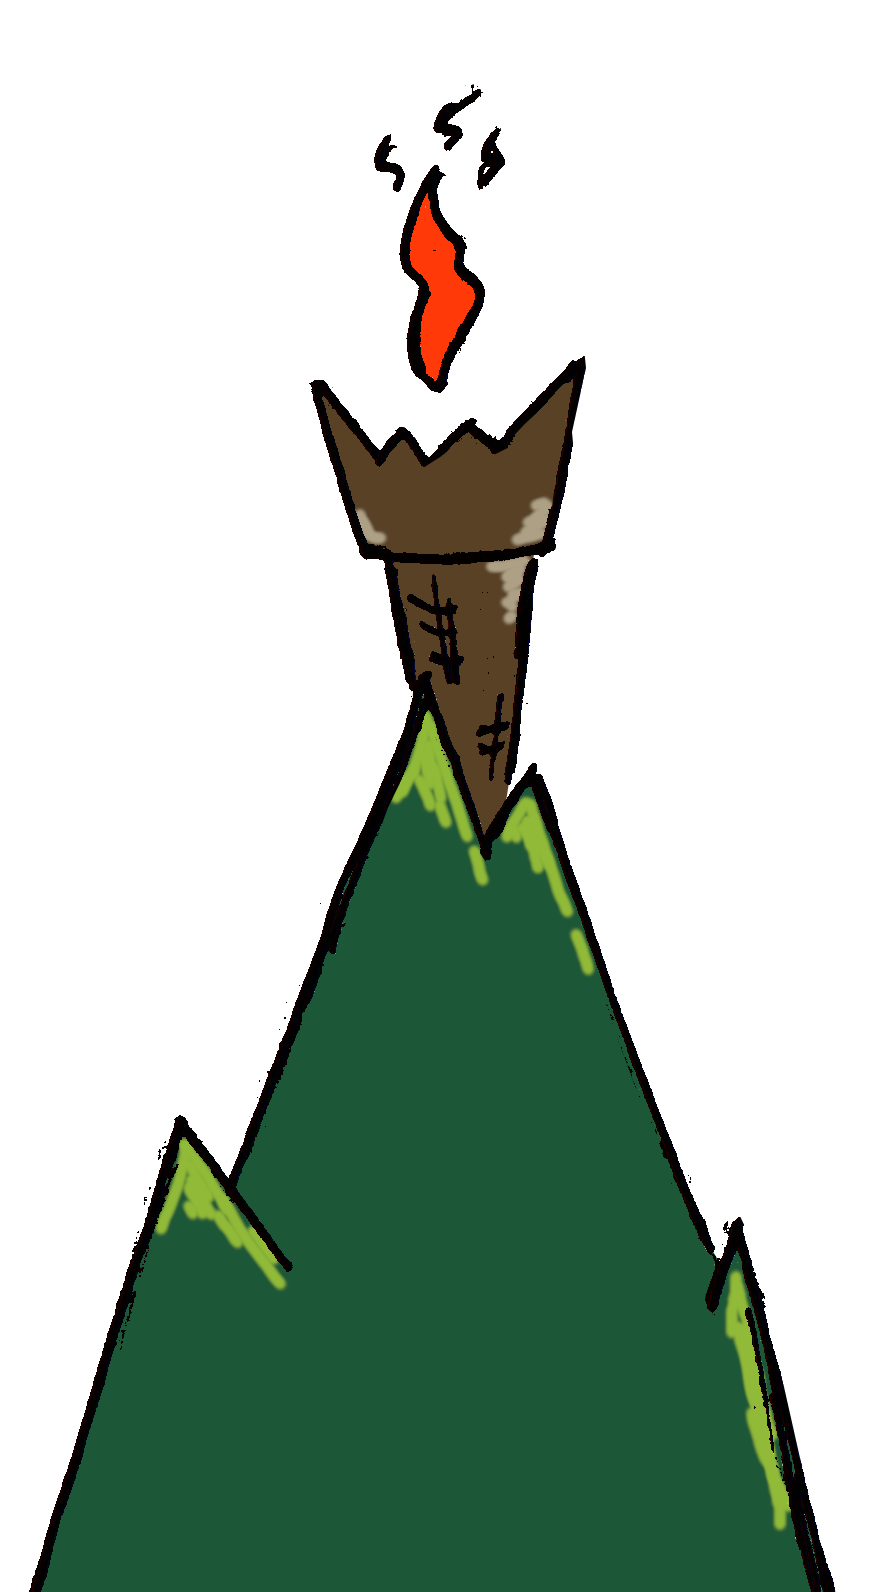
\includegraphics[width=9cm]{collina}};
			\draw [ultra thick, fill=earth!50!white] (9.5,3.5) rectangle (26.5,-3.5);
			\node (example-textwidth-2) [right, align=left, text width=16cm, color=black, font=\fontsize{18pt}{19pt}\selectfont] at (10,0) {Nel 1638, Galilei sugerì di misurare la velocità della luce utilizzando una lanterna posta sulla cima di una collina e quindi osservando il ritardo tra il momento in cui la lanterna viene coperta e quello in cui l'occhio percepisce tale evento. Il fisico pisano non riuscì a determinare se la luce viaggiasse istantaneamente o meno, ma concluse che in quest'ultimo caso doveva essere estremamente rapida.};
		\end{scope}
		%
		\begin{scope}[shift={(0,-21)}]
			\draw [ultra thick, fill=dida] (2.5,0) rectangle (28,-3.5);
			\node (example-textwidth-2) [right, align=left, text width=25cm, color=black, font=\fontsize{18pt}{19pt}\selectfont] at (3,-1.5) {La prima stima quantitativa della velocità della luce venne fatta da \textbf{Ole Rømer} nel 1676 a partire dalle osservazioni delle lune di Giove, in particolare Io. Egli stimò che la luce impiegava 22 minuti per percorrere il diametro dell’orbita terrestre.};
			\node at (7,-10) {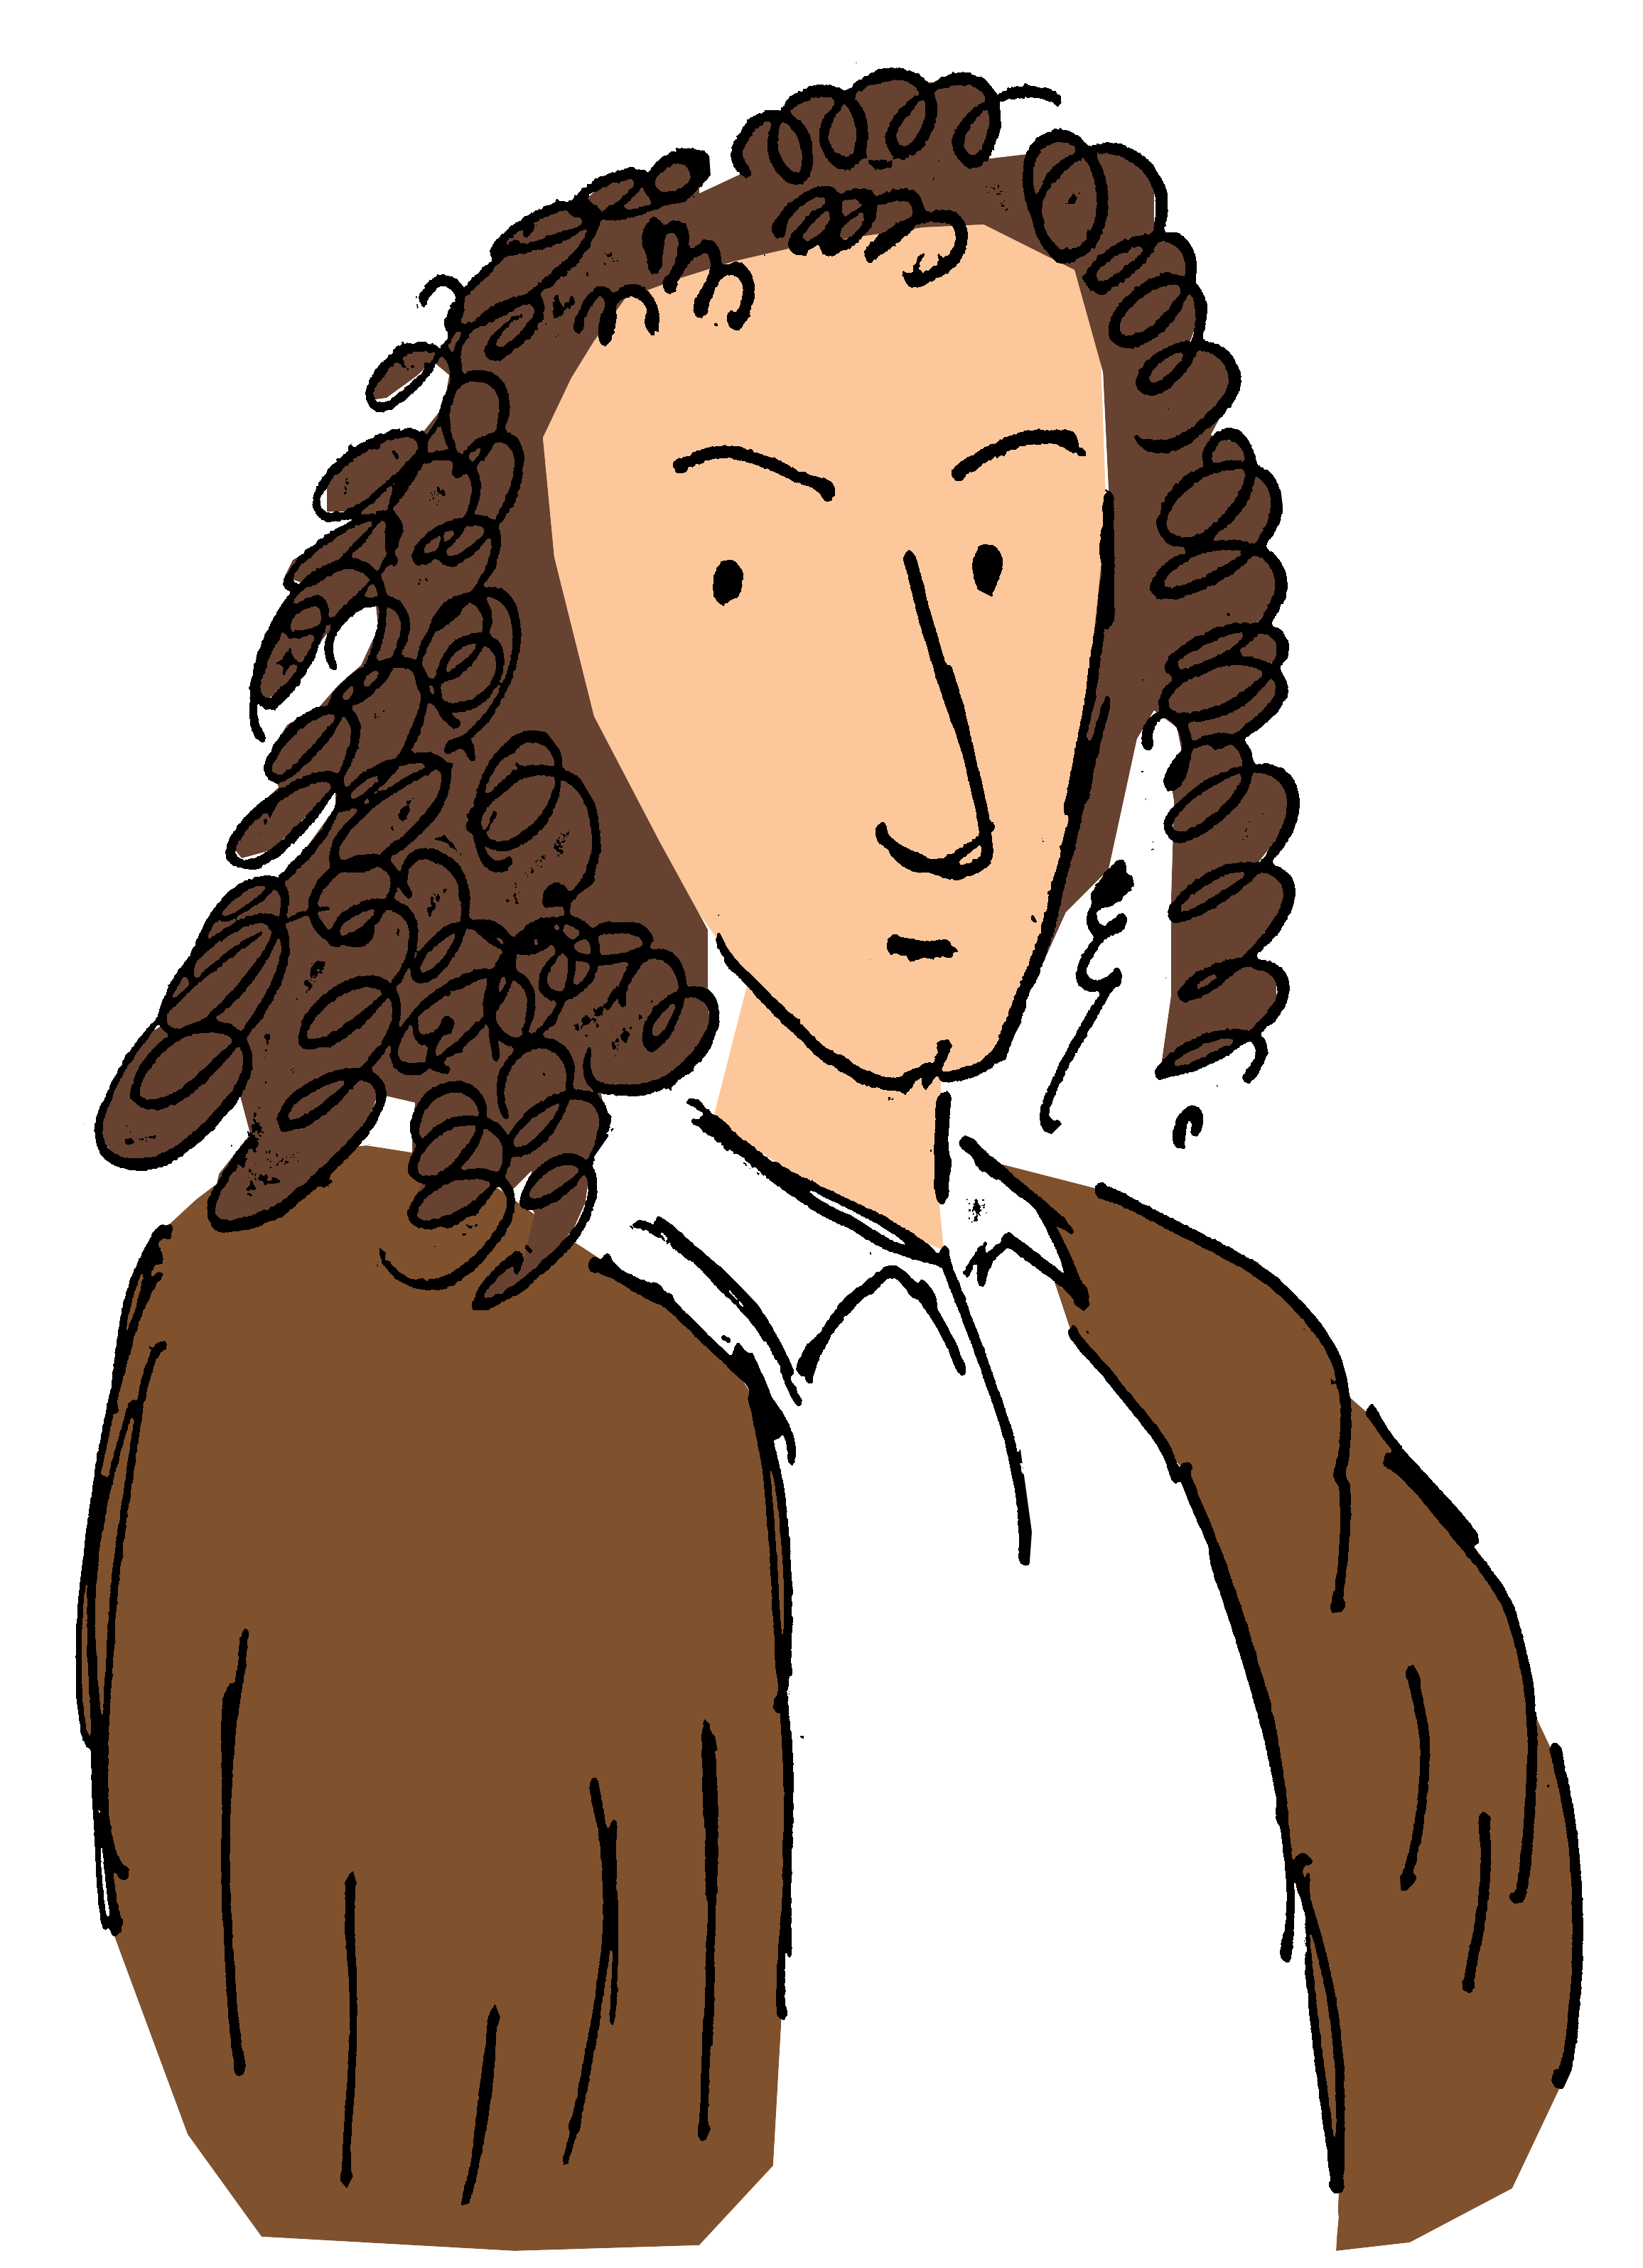
\includegraphics[width=8cm]{huygens}};
			\node (example-textwidth-2) [notice={(-3,0.5)}, ultra thick, right, align=center, text width=12cm, color=black, fill=white, font=\fontsize{23pt}{24pt}\selectfont] at (12,-11) {Utilizzando questa stima, io, \textbf{Christiaan Huygens}, ho stabilito in 220000 km/s la velocità della luce, ovvero circa il 26\% più bassa rispetto al valore reale.};
		\end{scope}
		%
		\begin{scope}[shift={(0,-43)}]
			\draw [ultra thick, fill=dida] (1.5,5) rectangle (26.5,-5);
			\node at (23,0) {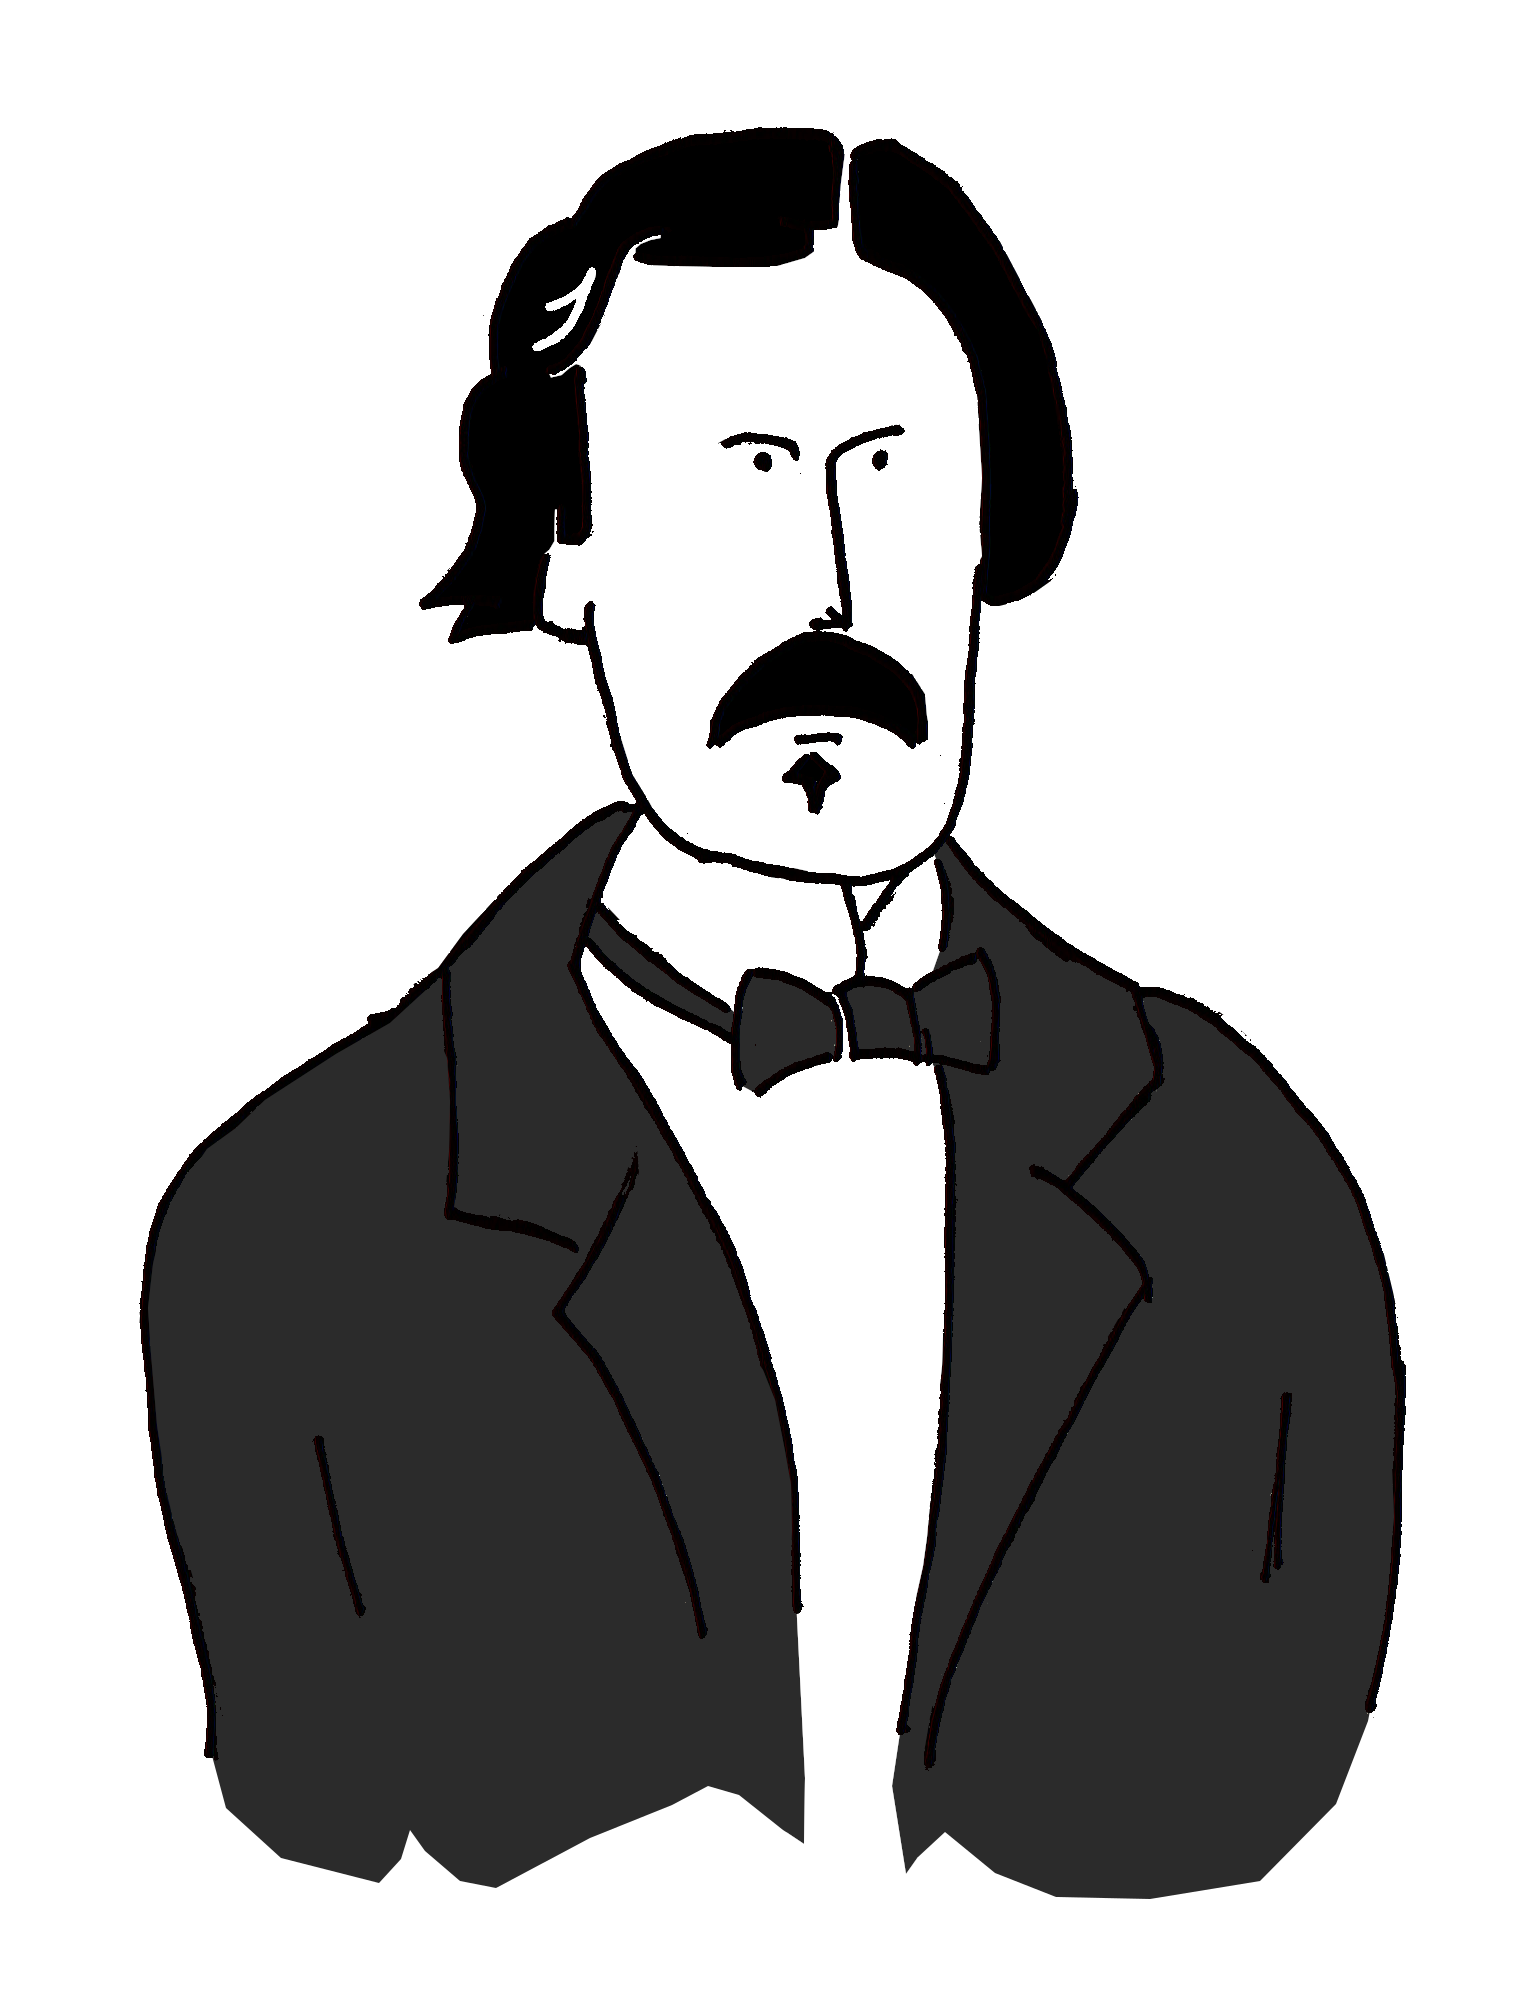
\includegraphics[width=10cm]{foucault}};
			\node (example-textwidth-2) [right, align=left, text width=16cm, color=black, font=\fontsize{18pt}{19pt}\selectfont] at (2,0) {Nel 1826 \textbf{Léon Foucault}, perfezionando il metodo della ruota dentata sviluppato da \textbf{Hippolyte Fizeau}, fornì un valore incredibilmente vicino a quello reale: 298000 km/s. Foucault utilizzò degli specchi rotanti, cosa che fecero anche \textbf{Albert Michelson} e \textbf{Edward Morley} nel 1887 in quello che è ancora oggi l’esperimento più famoso sulla determinazione dela velocità della luce, soprattutto perché giocò un ruolo fondamentale nella discussione più generale sull’etere e nello sviluppo della teoria della relatività ristretta.};
		\end{scope}
		%
		\begin{scope}[shift={(0,-51)}]
			\draw [ultra thick,fill=space] (4,1) rectangle (27,-1);
			\node (example-textwidth-2) [right, align=center, text width=25cm, color=white, font=\fontsize{23pt}{24pt}\selectfont] at (3,0) {Schema dell'esperimento di Michelson e Morley};
		\end{scope}
		% michelson morley
		\begin{scope}[shift={(15,-63)}]
			\draw [fill=moon] (0,0) circle (10cm);
			%
			\tkzDefPoint(0,0){O}
			\tkzDefPoint(-3,0.25){A} \tkzDefPoint(3,0.25){B}
			\tkzDefPoint(3,-0.25){C} \tkzDefPoint(-3,-0.25){D}
			%
			\tkzDefPointBy[rotation = center O angle 45](A) \tkzGetPoint{A1}
			\tkzDefPointBy[rotation = center O angle 45](B) \tkzGetPoint{B1}
			\tkzDefPointBy[rotation = center O angle 45](C) \tkzGetPoint{C1}
			\tkzDefPointBy[rotation = center O angle 45](D) \tkzGetPoint{D1}
			%
			\tkzDefPoint(-12,0){R1} \tkzDefPoint(-2,0){F1}
			\tkzDefPoint(8,0){R2} \tkzDefPoint(6,0){F2}
			\tkzDrawSegment[->](R1,F1)
			\tkzDrawSegment[->](F1,F2)
			\tkzDrawSegment[<-](F2,R2)
			\tkzDrawSegment(R1,R2)
			%
			\tkzInterLL(R1,R2)(A1,B1) \tkzGetPoint{M1}
			\tkzDefLine[orthogonal=through M1](R1,R2) \tkzGetPoint{E}
			%
			\tkzDefPoint(-3,8){A2} \tkzDefPoint(3,8){B2}
			\tkzDefPoint(-3,7.5){D2} \tkzDefPoint(3,7.5){C2}
			\tkzInterLL(M1,E)(C2,D2) \tkzGetPoint{M2}
			\tkzDrawSegment[->](M1,M2)
			%
			\tkzDefPoint(8,-3){A3} \tkzDefPoint(8.5,-3){B3}
			\tkzDefPoint(8.5,3){C3} \tkzDefPoint(8,3){D3}
			%
			\tkzInterLL(R1,R2)(C1,D1) \tkzGetPoint{M3}
			\tkzDefLine[orthogonal=through M3](R2,R1) \tkzGetPoint{F1}
			\tkzDefLine[orthogonal=through M1](R2,R1) \tkzGetPoint{F2}
			%
			\tkzDefPoint(-0.7,-9){a} \tkzDefPoint(0.7,-9){b}
			\tkzDefPoint(0.7,-11){c} \tkzDefPoint(-0.7,-11){d}
			\tkzInterLL(M3,F1)(a,b) \tkzGetPoint{f1}
			\tkzDrawSegment[->](M3,f1)
			\tkzInterLL(M1,F2)(a,b) \tkzGetPoint{f2}
			\tkzDrawSegment[->](M1,f2)
			\tkzDrawPolygon[fill=white](a,b,c,d)
			%
			\tkzDrawPolygon[fill=earth,opacity=0.5,ultra thick](A1,B1,C1,D1)
			\tkzDrawPolygon[fill=earth,opacity=0.5,ultra thick](A2,B2,C2,D2)
			\tkzDrawPolygon[fill=earth,opacity=0.5,ultra thick](A3,B3,C3,D3)
			%
			\node at (0,8.5) {\textcolor{black}{\fontsize{15}{16}\selectfont specchio}};
			\node at (-4.5,0.5) {\textcolor{black}{\fontsize{15}{16}\selectfont raggio di luce coerente}};
			\node[left] at (8.5,3.5) {\textcolor{black}{\fontsize{15}{16}\selectfont specchio}};
			\node at (-3.5,-2.5) {\textcolor{black}{\fontsize{15}{16}\selectfont specchio}};
			\node at (-3.5,-3.1) {\textcolor{black}{\fontsize{15}{16}\selectfont semitrasparente}};
			\node[left] at (-0.7,-10.5) {\textcolor{black}{\fontsize{15}{16}\selectfont rilevatore}};
		\end{scope}
		%
		\begin{scope}[shift={(0,-79)}]
			\draw [ultra thick, fill=earth] (4.5,4) rectangle (9.5,-4);
			\node at (7,0) {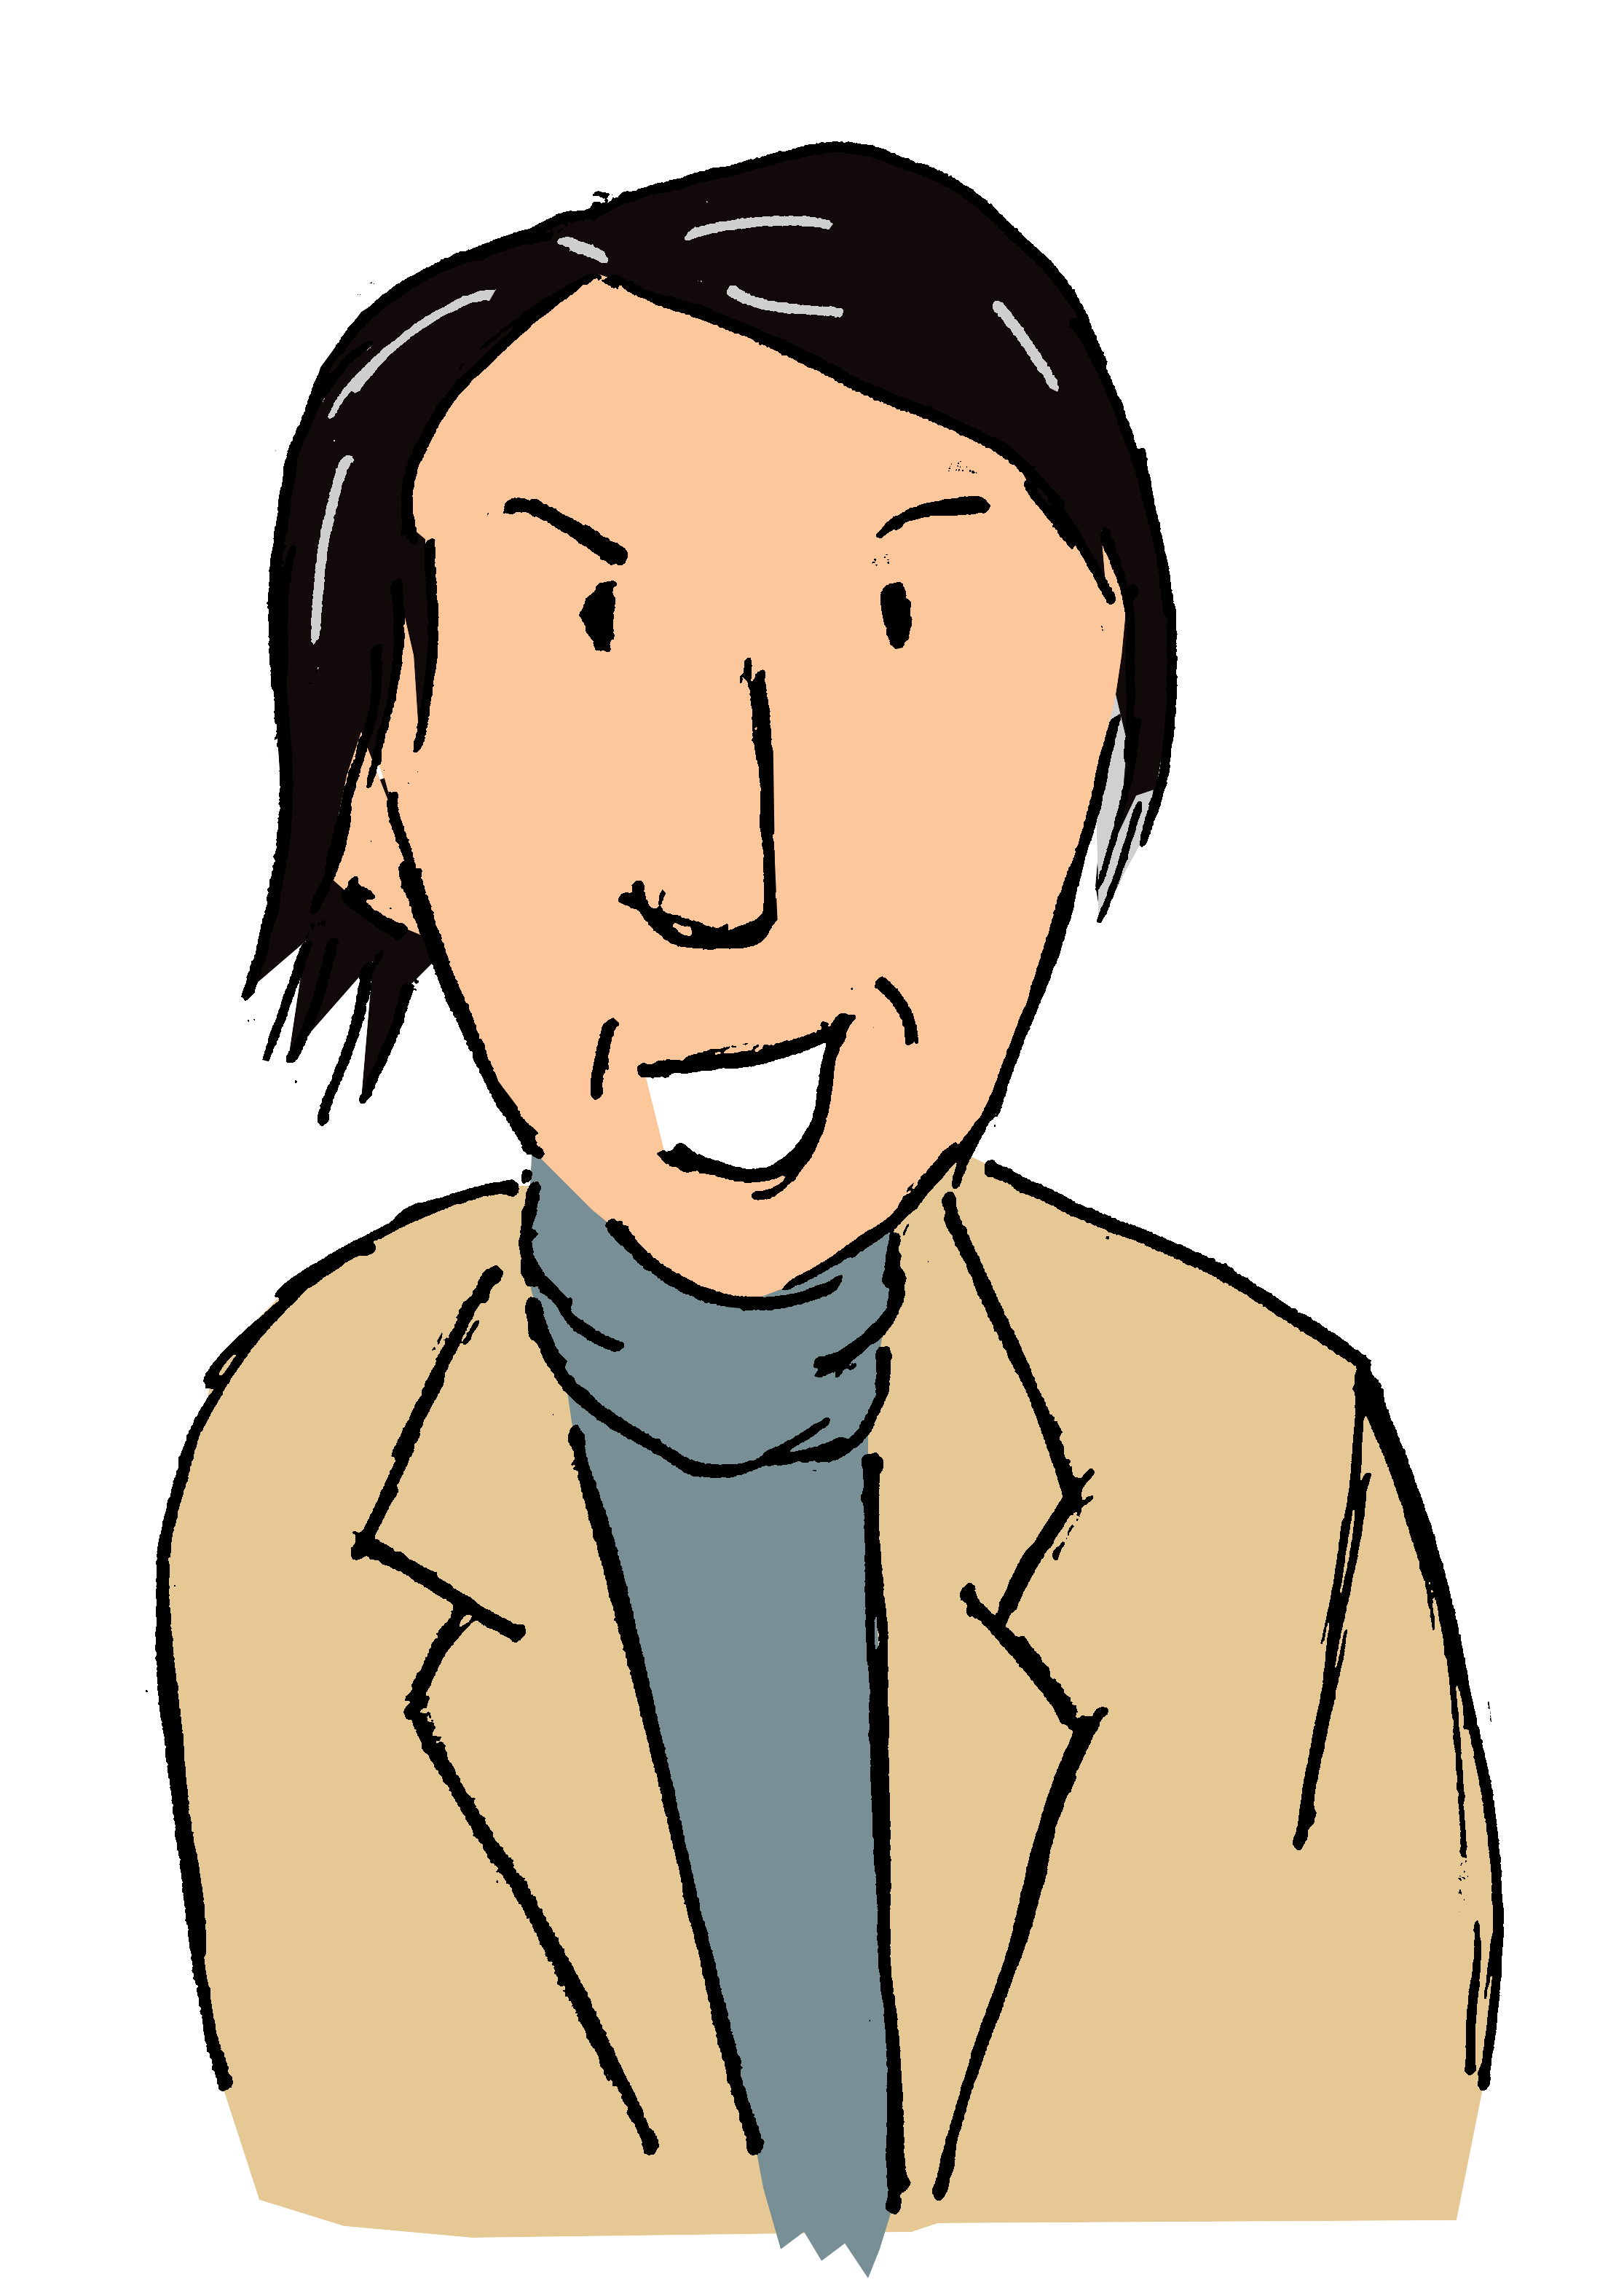
\includegraphics[width=5cm]{carl_sagan}};
			\node (example-textwidth-2) [notice={(-3,0.5)}, ultra thick, right, align=center, text width=12cm, color=black, fill=white, font=\fontsize{23pt}{24pt}\selectfont] at (12,-1) {Nel 1983 la 17.ma Conferenza Generale sui pesi e le misure stabilì per la velocità della luce nel vuoto il valore costante di 299792458 m/s, rendendo così la luce una costante all’interno del sistema internazionale di misure.};
		\end{scope}
		%
		\begin{scope}[shift={(0,-87)}]
			\node at (27,0) () {
\includegraphics[width=3.7cm]{licenza}};
			\node at (18,-0.1) {\textcolor{black}{\fontsize{14}{15}\selectfont Testo e illustrazioni: @ulaulaman - Gianluigi Filippelli}};
		\end{scope}
	\end{tikzpicture}
%
\end{document}
